\section{Method}

\subsection{Problem Formulation}

The purpose of this paper is to design a learnable quantum circuit for quantum computers with a similar architecture to the Transformer Encoder, and to explore how much improvement such a model can achieve.
Sequence-to-sequence learning is about training models to convert sequences from one domain to sequences in another domain. Using sequence-to-sequence model as backbone can also adapt the model to other tasks, such as text classification and image classification.

The methods of this paper are proposed under the following assumption.
\begin{itemize}
  \item There is a concept processing unit called QPU (Quantum Processing Unit), which is a NISQ device that can is connected to a classical computer. QPU can compute any basic quantum rotation gate and entanglement gate in $O(1)$ time complexity.
  \item There is a limited number of qubits on the QPU, for example, 32 qubits on the QPU.
  \item The inputs of the model will have the same length or can be chopped and padded into the same length.
\end{itemize}

The challenge to build a sequence-to-sequence learning model on current NISQ device is that the model has to utilize low number of qubits and shallow circuit. The development of NISQ device has made rapid progress recently; in 2021, IBM released the “Eagle” quantum computer, which has 127 qubits, making it the largest quantum computer at the time. However, it is still difficult to fit a classical sequence-to-sequence machine learning model into the size of a quantum computer. Even if it can, there is no obvious advantage to train the model on a quantum computer. In this work, We aim to propose an NLP model that is optimized for quantum computer and experiment on the NISQ device that is currently available.

\subsection{Architecture}

\begin{figure}[htp!]
  \centering
    \tikzstyle{layer} = [draw, text centered, text width=14em, minimum height=2em, rounded corners]
    \tikzstyle{ffblock} = [layer, fill=cyan!30]
    \tikzstyle{attnblock} = [layer, fill=orange!30]
    \tikzstyle{measure} = [layer, fill=green!10]
    \tikzstyle{encode} = [layer, fill=red!20]
    \tikzstyle{params} = [layer, fill=red!20]
    \begin{tikzpicture}
        \node (output) [text centered, text width=14em] {Outputs};
        \node (measure) [measure] [below of=output] {Pauli-Z Measurement};
        \node (ffblock) [ffblock] [below of=measure] {Simplified Quantum Feedforward};
        \node (attn) [attnblock] [below of=ffblock] {Quanttention};
        \node (encode) [encode] [below of=attn] {Input Encoding};
        \node (parameters) [params] [below of=encode] {Parameters Layer};
        \node (input) [text centered, text width=14em] [below of=parameters] {Inputs};
        
        \begin{scope}[on background layer]
            \node [fill=cyan!20, rounded corners, fit={(encode) (attn) (ffblock) (measure) }] {};
            \node [fill=orange!20, rounded corners, fit={(input) (parameters)}] {};
            \node [fill=orange!20, rounded corners, fit={(output)}] {};
            \node [draw, densely dashed, rounded corners, fit={(attn) (ffblock)}, label={right:$\times N$}] {};
            
            \draw[->] (input) -- (parameters);
            \draw[->] (parameters) -- (encode);
            \draw[->] (encode) -- (attn);
            \draw[->] (attn) -- (ffblock);
            \draw[->] (ffblock) -- (measure);
            \draw[->] (measure) -- (output);
        \end{scope}
        
        \matrix [draw,above] at ($(output)+(0, 0.8)$) {
          \node [fill=orange!20, rounded corners, label=right:Classical Computer] {}; \\
          \node [fill=cyan!20, rounded corners, label=right:Quantum Computer] {}; \\
        };
    \end{tikzpicture}
  \caption{The QNet Encoder Block Architecture.}
  \label{fig:qnet-encoder}
\end{figure}

In this section, we will describe the concept of QNet and purpose a residual connected QNet (ResQNet) which use QNet as its main component.

The concept of QNet can be separated into 3 parts. First, the word embedding is encoded onto a quantum computer. Second, a learnable word vector transformation and a token mixing mechanism are applied repeatedly to learn the representation of the combination of words. Finally, the measurement is applied on every qubit to take the quantum state back to classical computer. Since the result will be a flattened tensor, it has to be reshaped back to the original input shape.

The concept of QNet is simple. However, the actual process of QNet encoder is more complex and shown in Fig.~\ref{fig:qnet-encoder}. The quantum circuit has to be constructed for quantum compute before the execution. The parameters of word embedding and learnable word vector transformation have to be coded onto the circuit. The Parameters Layer in the figure prepares the parameters needed by the quantum circuit. The Input Encoding layer in the figure maps the word embedding into each qubit. The Quanttention layer introduces the mechanism to relate each token with others. The Simplified Quantum Feedforward Layer performs learnable unitary transformation on each token. The Quanttention layer and Simplified Quantum Feedforward layer can be repeated multiple times to mix the tokens more evenly. The QNet is only used to generate encoded representation. We will still use classical neural network to project the result of QNet into output space. To take the quantum data back to the classical computer, the Pauli-Z observable is used to measure the computed qubits.

\begin{figure}[htp!]
  \centering
    \tikzstyle{layer} = [draw, text centered, text width=14em, minimum height=2em, rounded corners]
    \tikzstyle{denseblock} = [layer, fill=violet!10]
    \tikzstyle{outputblock} = [layer, fill=blue!10]
    \tikzstyle{qnet} = [layer, fill=green!10]
    \tikzstyle{encode} = [layer, fill=red!20]
    \begin{tikzpicture}
        \node (output) [outputblock] {Output Projection};
        \node (dense) [denseblock] [below of=output] {Linear};
        \node (add) [font=\Large] [below of=dense] {$\oplus$};
        \node (qnet) [qnet] [below of=add] {QNet Encoder};
        \node (begin) [] [below of=qnet] {};
        \node (encode) [encode] [below of=begin] {Embedding Layer};
        
        \begin{scope}[on background layer]
            \node [draw, densely dashed, rounded corners, fit={($(begin)-(3.5, 0.2)$) ($(add)+(3.5, 0.2)$)}, label={right:$\times N$}] {};
            \draw[->] (encode) -- (qnet);
            \draw[->] (qnet) -- (add);
            \draw[->] (add) -- (dense);
            \draw[->] (dense) -- (output);
            
            \draw[->] (begin) -- ($(begin)+(3,0)$) -- ($(add)+(3,0)$) -- (add);
        \end{scope}
        
    \end{tikzpicture}
  \caption{The ResQNet - the model architecture.}
  \label{fig:resqnet}
\end{figure}

The ResQNet is a model that is composed by multiple residual connected QNet blocks, as shown in Fig.~\ref{fig:resqnet}. It is a feasible model for NISQ device and temporary replacement of quantum-native residual neural network since residual neural network is hard to implement on NISQ.

The derivation and circuit design are introduced in details in the following sections.

\subsubsection{Word Embedding Quantum Encoding}
The goal of the word embedding model is to map each token in the corpus into a $d$-dimensional vector with each dimension representing at least one meaning, that is, $f: [d] \rightarrow R^d$. 

In Transformer, the word embedding is added with \emph{positional encoding}. It is to make use of positional information in the model. In this work, we do not add the positional encoding to the word embedding. Instead, we utilize the property of qubits as follows.

We use two axes of qubits to encode data into the quantum computer. Word embeddings are transformed to the volume of a qubit, that is, the angle on Pauli-X. Thus, the range of numbers in the word embedding layer will fall in $[0, 2\pi)$. The position of the word is encoded as the phase of the qubit, that is, the angle on Pauli-Z. The angle of position information ranges in $[0, \pi)$. The transformation can be described as Equation~\ref{equ:word_embedding}. In the equation, $x$ is the input token array, and the superscript denote the index of the token and the subscript denote the index of the embedding. $n$ is the length of the input sequence, $d$ is the embedding dimension. This method can be visualized via the Bloch sphere as shown in Fig.~\ref{fig:word-sphere}.

\begin{equation} \label{equ:word_embedding}
x \rightarrow |\psi_x\rangle = ( \prod_{i=1}^n \prod_{j=1}^d R_x( \frac{(i-1) \pi}{n} )R_z(x^i_j) ) |0\rangle
\end{equation}

\begin{figure}[htp!]
    \centering
    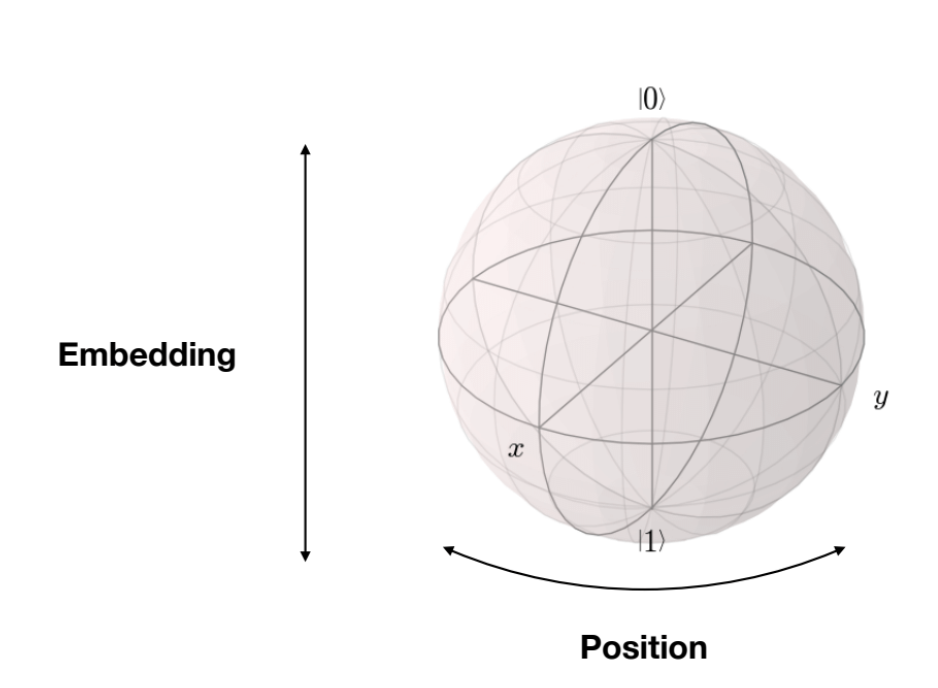
\includegraphics[width=7cm]{images/word-sphere.png}
    \caption{The Bloch sphere illustration of Word Embedding Quantum Encoding on a single qubit.}
    \label{fig:word-sphere}
\end{figure}

\begin{figure}[htp!]
  \centering
    \Qcircuit @C=2em @R=.7em {
    & |0 \rangle & & \gate{R_x(0)} & \gate{R_z(x^1_1)} & \qw & |\psi_1 \rangle & \\
    & |0 \rangle & & \gate{R_x(0)} & \gate{R_z(x^2_1)} & \qw & |\psi_1 \rangle & \\
    & |0 \rangle & & \gate{R_x(\frac{\pi}{2})} & \gate{R_z(x^1_2)} & \qw & |\psi_2 \rangle & \\
    & |0 \rangle & & \gate{R_x(\frac{\pi}{2})} & \gate{R_z(x^2_2)} & \qw & |\psi_2 \rangle & \\
    }
  \caption{The quantum circuit of Word Embedding Quantum Encoding for 2 words with 2 embedding.}
  \label{fig:embedding}
\end{figure}

\subsubsection{Quanttention}
A self-attention mechanism is an attempt to implement the action of selectively concentrating on a few relevant things, while ignoring others in deep neural networks~\cite{}.

In this work, we demonstrate why dot-product attention cannot be applied and propose a possible solution to implement the similar behavior. This solution considers the quantum computer resource on hand.

Since qubits are precious in the current stage NISQ, we do not want to use auxiliary qubits in this submodule. It is impractical to do the dot-product attention in the current scale of NISQ devices. For instance, the circuit of quantum state dot-product is shown in Fig.~\ref{fig:dot-product}. $\theta_1$ and $\theta_2$ are sets of learnable parameter for rotation gates in VQE. After the dot-product operation, $|\psi_1\rangle$ and $|\psi_2\rangle$ will be corrupted and cannot be recovered to the same state as before. Therefore, each time when the dot product is computed, the quantum state needs to be duplicated. There are at least $O(n \times d)$ dot-products, so this method is not feasible in the current NISQ device.

\begin{figure}[htp!]
  \centering
    \Qcircuit @C=2em @R=.7em {
    & |\psi_1 \rangle & & \gate{VQE(\theta_1)} & \qswap & \qw & \qw \\
    & |\psi_2 \rangle & & \gate{VQE(\theta_2)} & \qswap & \qw & \qw\\
    & |0\rangle & & \gate{H} & \ctrl{-2} & \gate{H} & \qw \\
    }
  \caption{The quantum circuit of Dot-Product with 2 quantum encoded word embedding.}
  \label{fig:dot-product}
\end{figure}


In FNet~\cite{}, the attention mechanism can be presented as Equation~\ref{equ:fnet}, in which $x$ is the input sentence while $F_h$ and $F_{seq}$ are Fast Fourier Transform on embedding dimension and sequence dimension, respectively. The results of FNet are approximately the same as the original multi-head attention.

\begin{equation} \label{equ:fnet}
y =  L_2(\mathbf{R}(F_{seq}(F_h(x))))
\end{equation}

If the purpose to perform the Fourier transform is just to \emph{mix} the tokens, the transformation can be simplified by removing the Fourier transform on the embedding dimension into Equation~\ref{equ:fnet-simple}.

\begin{equation} \label{equ:fnet-simple}
y = L_2(\mathbf{R}(F_{seq}(x)))
\end{equation}

By the concept of Equation~\ref{equ:fnet-simple}, we design the Quanttention mechanism. The unitary of Quantum Fourier Transform on the $i$-th embedding is presented in Equation~\ref{equ:u_qft}. In the equation, $n$ is the length of the input sentence and the $N$-th root of unitary is defined as $\omega^{jk}_N = e^{2\pi i \frac{jk}{N}}$.

\begin{equation} \label{equ:u_qft}
U_{QFT_i} = \frac{1}{\sqrt{n}} \sum_{j=0}^{n-1}  \sum_{k=0}^{n-1} \omega _{n}^{jk} |ki\rangle \langle ji|
\end{equation}

The Quanttention mechanism employs this unitary for each embedding. The formula is shown as Equation~\ref{equ:quanttention}. In the equation, $d$ is the embedding dimension.
 
\begin{equation} \label{equ:quanttention}
|y\rangle = U_{QFT_1}\ldots U_{QFT_d}|\psi\rangle
\end{equation}

Therefore, Quanttention is made up of Quantum Fourier Transforms performed on all tokens for each qubit in the embedding. The trainable quantum circuit is shown in Fig.~\ref{fig:quanttention}.

\begin{figure}[htp!]
  \centering
    \Qcircuit @C=2em @R=.7em {
    & |\psi^1_1 \rangle & & \qw & \multigate{1}{\ \mathcal{QFT}\ } & \qw & \qw \\
    & |\psi^2_1 \rangle & & \qswap & \ghost{\ \mathcal{QFT}\ } & \qswap & \qw \\
    & |\psi^1_2 \rangle & & \qswap \qwx & \multigate{1}{\ \mathcal{QFT}\ } & \qswap \qwx & \qw\\
    & |\psi^2_2 \rangle & & \qw & \ghost{\ \mathcal{QFT}\ } & \qw & \qw
    }
  \caption{Quanttention circuit.}
  \label{fig:quanttention}
\end{figure}


\subsubsection{Simplified Quantum Feedforward Network}

Quantum neural networks are known to have a three-dimensional architecture, with each neuron represented by a qubit. Because entanglement prevents the qubit from being reused, deep quantum neural networks are difficult to create with the existing NISQ technology.

Since the goal of this work is to construct a viable machine learning model, the Feedforward layer cannot include auxiliary qubits. Hence, the quantum neural network must be simplified. The circuit is shown in Fig.~\ref{fig:feedforward}

\begin{figure}[htp!]
  \centering
    \Qcircuit @C=2em @R=.7em {
    & |\psi^1_1 \rangle & & \multigate{1}{VQE(\theta_1)} & \multigate{1}{\ \mathcal{G}\ }& \multigate{1}{VQE(\theta_2)} & \qw \\
    & |\psi^2_1 \rangle & & \ghost{VQE(\theta_1)}& \ghost{\ \mathcal{G}\ } & \ghost{VQE(\theta_2)} & \qw \\
    }
  \caption{Simplified Quantum FeedForward with single vocab and 2 wires.}
  \label{fig:feedforward}
\end{figure}

In a typical transformer architecture, the Feedforward layer has two fully connected layers with one activation function between them. In the Simplified Quantum Feedforward layer, a similar arrangement is utilized, with two VQE separated by an activation function $\mathbf{G}$. The process can be demonstrated as Equation~\ref{equ:Feedforward}.

\begin{equation} \label{equ:Feedforward}
|\hat{\psi^1}\ldots\hat{\psi^m}\rangle = U_1U_\mathbf{G}U_2|\psi^1\rangle \ldots U_1U_\mathbf{G}U_2|\psi^m\rangle
\end{equation}

The objective of an activation function is to prevent gradient vanishing in a deep neural network model. It may be used millions of times, thus it must be computationally efficient.
The $\mathbf{G}$ is an amplitude amplification operator, which means that when the amplitude of a quantum state $|\psi\rangle = \sum^{2^{n}}_{i=1} x_i$ is described as $|x_i|^2$, the amplitude amplification operator will polarize the amplitudes. The unitary of $\mathbf{G}$ is expressed in Equation~\ref{equ:U_G}.

% Prove G operator by graph

\begin{equation} \label{equ:U_G}
U_\mathbf{G} = H^{\otimes m}(2|\psi\rangle\langle \psi|- I)H^{\otimes m}
\end{equation}

The circuit of $\mathbf{G}$ is shown in Fig.~\ref{fig:g-operator}.

\begin{figure}[htp!]
  \centering
    \Qcircuit @C=2em @R=.7em {
    & |\psi^1_1 \rangle & & \gate{H} & \ctrl{1} & \gate{H} & \qw \\
    & |\psi^2_1 \rangle & & \gate{H} & \ctrl{1} & \gate{H} & \qw \\
    & |\psi^3_1 \rangle & & \gate{H} & \targ & \gate{H} & \qw \\
    }
  \caption{Circuit of $\mathbf{G}$}
  \label{fig:g-operator}
\end{figure}

\subsubsection{Measurement}
In the end, quantum measurements on Pauli-Z are performed for every qubit. The measured result is a 1-D tensor with all entries lie in $[-1, 1]$. In order to pass the output into next block, that is, making the QNet as a sequence to sequence model. Tensor are shaped to the shape before entering the QNet.
